\chapter{Magnetic Field and Magnetic Forces}
So far we have discussed electric fields $\vec{E}$, which give force $\vec{F}_E = q \vec{E}$ on a charge $q$, no matter what its velocity. But the electromagnetic field also includes another vector field, the magnetic field $\vec{B}$, which gives a force $\vec{F}_B = q\vec{v} \times \vec{B}$ on a charge $q$ that depends on its velocity $\vec{v}$ and is zero if the velocity is zero. 

The magnitude of the magnetic force is 
\begin{equation}
F_B = \abs{\vec{F}_B} = \abs{q\vec{v}\times \vec{B}} = \abs{q}v_\perp B = \abs{q}vB \sin \theta,
\end{equation}
where $v_\perp = v \sin \theta$ is the component of the velocity perpendicular to $\vec{B}$. $\vec{F}_B$ is perpendicular to both $\vec{v}$ and $\vec{B}$ and with the sense that one's right thumb would point if one's fingers coiled from first being in the direction of $\vec{v}$ and then towards the tips in the $\vec{B}$ direction. 

\begin{wrapfigure}{R}{5cm}
\centering
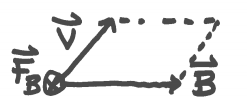
\includegraphics[width=5cm]{Images/chap7_1.png}
\end{wrapfigure}

$\vec{v} \times \vec{B}$ has magnitude $\vec{v}$ and $\vec{B}$. It is the vector `area' $\vec{A} = \vec{v} \times \vec{B}$ associated with this parallelogram, perpendicular to the area itself. In this case the vector $\vec{v} \times \vec{B}$ points into the page (or screen when the image is projected), as indicated by $\otimes$, which symbolizes the tail feathers of an arrow pointing away. The opposite arrow perpendicular to the paper, say $-\vec{v} \times \vec{B} = \vec{B} \times \vec{v}$, would be indicated by $\odot$, which symbolizes the tip of an arrow pointing toward the viewer.

The sense can also be given by the direction the tip of a screw would move if it's axis were perpendicular to $\vec{v}$ and $\vec{B}$ and its head (parallel to the plane of $\vec{v}$ and $\vec{B}$) were turned by $<180\deg$ from $\vec{v}$ to $\vec{B}$.

When both an electric field $\vec{E}$ and a magnetic field $\vec{B}$ is present, the total electromagnetic field force on a particle of charge $q$ and velocity $\vec{v}$ is called the \textbf{Lorentz force},
\begin{equation}
\boxed{\vec{F} = q(\vec{E} + \vec{v} \times \vec{B})}.
\end{equation}

Electric fields are produced by charges whether or not they are moving (though the electric fields deviate from Coulomb's law if the charges are accelerating or have velocities comparable to the speed of light, $\SI{299792456}{\frac{m}{s}}$), but magnetic fields are produced only by charges that are moving and/or accelerating. Later we shall discuss the analogues of Coulomb's law for how magnetic fields are produced. Charges moving within atoms and molecules are one way. Another is that even a charge not moving can have a spin, which produce a dipole magnetic field.

Just as the electric field $\vec{E}$ has electric field lines that are everywhere parallel to $\vec{E}$ and that give a flux $\Phi_E = \oint \vec{E} \cdot \di \vec{A}$ through a surface, so a magnetic field $\vec{B}$ has \textbf{magnetic field lines} everywhere parallel to $\vec{B}$ and that give a flux $\Phi_B = \int \vec{B} \cdot \di \vec{A}$ through a surface. For the electric field, Gauss's law gives the electric flux outward through a closed surface as 
\begin{equation}
\Phi_E = \oint \vec{E} \cdot \di \vec{A} = \frac{Q_{encl}}{\varepsilon_0},
\end{equation}
where $Q_{encl}$ is the total electric charge inside the volume enclosed by the surface. The analogue for the magnetic field would be $\Phi_B = \oint \vec{B} \cdot \di \vec{A} \propto$ (magnetic charge $Q_B$ enclosed). However, no magnetic charge $Q_B$ has ever been observed, so we shall say Gauss's law for magnetism is $\boxed{\oint \vec{B} \cdot \di \vec{A} = 0}$ through any closed surface.

Analogous to the way that Maxwell in 1865 completed the development of \textbf{electromagnetism} started by Coulomb, Gauss, Ampere, Faraday, and others, the 1960s saw the unification of electromagnetism and the \textbf{weak interaction} (radioactivity) by Glashow, Weinberg, and Salam. When combined with the theory of \textbf{quantum chromodynamics} for the strong nuclear reactions, including the Higgs mechanism for generating the masses of quarks (the building blocks for hadrons such as protons and neutrons) and of electrons and related other leptons, this gives what is known as the \textbf{Standard Model} of particle physics. However, this treats rather separately, and does not fully unify, the \textbf{electroweak} and \textbf{strong} interactions. Such a unification would be a \textbf{Grand Unified Theory}.

Such a \textbf{Grand Unified Theory} (GUT) would explain why the electron charge seems to be exactly the same magnitude (but opposite sign) as the proton charge, and, related to this, it predicts the existence of \textbf{magnetic monopoles}, which would have nonzero magnetic charge. However, these magnetic monopoles are predicted to have energies about a trillion times larger than the energies that can be produced in the largest accelerator today, the \textbf{Large Hadronic Collider (LHC)} at CERN, where several UofA professors work. So unless these estimates are wrong, it might be too difficult for humans ever to produce magnetic monopoles. Therefore, in this course we shall assume $\oint \vec{B} \cdot \di \vec{A} = 0$ or no magnetic monopoles.

\textbf{Gauss's Law for magnetism with no magnetic monopoles}, or $\boxed{\oint \vec{B} \cdot \di \vec{A} = 0}$, implies that magnetic field lines have no beginning or end. Generally, they come in from infinity and go back out to infinity, but they can also wrap around and around in a finite volume without ever reconnecting, unlike what the textbook says near the bottom of p.889: ``Like all other magnetic field lines, they form closed loops." Only in special situations, such as symmetry of rotation about an axis, or other situations in which a set of field lines stay in one plane without going to infinity, do the field lines form closed loops.

Asymmetric field lines do not stay on any single non-branching surface, and they need not form closed loops. A permanent magnet longer along the direction of the magnetic field inside has a north pole end (N) and a south pole end (S). Magnetic field lines run through the magnet from the S end to the N end and then emerge to loop back outside (though) they need not stay in a plane or distorted plane to reconnect precisely). However, because magnetic field lines nowhere begin or end, if one cuts the magnet in two, one will not get an isolated north pole or south pole, but rather the two new magnets will each have a north pole end and a south pole end, with the magnetic field passing through each magnet from south to north and then looping back outside, without ever ending.

A compass needle is a magnet free to rotate in the horizontal plane (when the compass is level), and then the north pole end of the compass points in the direction of the horizontal component of the magnetic field. From a Natural Resources Canada magnetic declination calculator online, when I entered the date 2019 March 12 and latitude $\frac{\pi}{2} - \frac{2}{\pi}$ radians = $\ang{53.5244}$N and longitude $\frac{5\pi}{6} - \frac{2}{\pi}$ radians = $\ang{113.5244}$W for the University of Alberta (``colatitude equator's reciprocal", and longitude $\pi/3 = \ang{60}$ greater than latitude), 1 got a magnetic declination of $\ang{14.094}$E, meaning that a compass would point $\ang{14.094}$ east of true north. It also said that this declination is decreasing about $\ang{1.04}$ every 6 years. Where I lived in Manokotak, Alaska, the declination decreased from $\ang{20}$E when I first went there in late summer 1959 to $\ang{12.2}$E today, a decreased of $\ang{7.8}$ in 60 years, an average decrease of $\ang{0.13}$/year or $\ang{1}$/(8 years).

The earth itself acts like a relatively permanent magnet, though its magnetic field is gradually changing with time (for example, with the North Magnetic Pole, where $\vec{B}$ is vertically downward, moving across northern Canadian islands during my lifetime, now being north of the Canadian Arctic territorial claim and within $\ang{4}$ of the Geographic North Pole and moving toward Russia at 55-60 km/year) and also reverses at random time intervals ranging between 100000 years and 50000000 years, the most recent being about 780000 years ago.

The earth's magnetic field is crudely a dipole field, with the dipole part having an axis that passes through the North Geomagnetic Pole that in 2015 was located at $\ang{80.37}$N, on Ellesmere Island, Nunavut, Canada. But because the field is not purely a dipole, the North Magnetic Pole and the North Geomagnetic Pole do not coincide, and a compass needle does not point to either.

When two magnets are placed close together end to end, the magnetic field energy is lower if the magnetic field on the axis is aligned: $\boxed{\text{S} \rightarrow \text{N}}$  $\boxed{\text{S} \rightarrow \text{N}}$ Thus the north pole of one magnet attracts the south pole of another, so opposite poles attract, rather similar to the way opposite charges attract and charges of the same sign repel, except that for magnets, one cannot have isolated poles. But since the north pole of a compass is attracted towards the north magnetic pole of the earth (where the magnetic field enters the earth vertically downwards), if one views the earth as a magnet, the North Magnetic Pole, or perhaps slightly better, the North Geomagnetic Pole (intersection of the dipole axis with the earth in the north), is a magnetic south pole, where magnetic field lines enter the earth, as they do in the south pole of a magnet.

Since the magnetic force magnitude is
\begin{equation}
F_B = \abs{\vec{F}_B} = \abs{q \vec{v} \times \vec{B}} = \abs{q} v_\perp B = \abs{q} v B_\perp ,
\end{equation}
the units of magnetic field are those of $\frac{F}{qv} = \SI{}{\frac{kg \cdot m/s^2}{C \cdot m/s} = \SI{}{\frac{kg}{C \cdot s}} = \SI{}{\frac{kg}{A \cdot s^2}} = \SI{}{T}}$, the \textbf{tesla}, (in honor of Nikola Tesla, 1856-1943, the prominent Serbian-American scientist and inventor). $\SI{1}{T} = \SI{1}{\frac{kg}{A \cdot s^2}} = \SI{1}{\frac{N}{A \cdot m}}$. 

Another common unit is the \textbf{gauss (G)}, $\SI{1}{G} = \SI{e-4}{T}$, a more convenient unit for the earth's magnetic field, since over the earth's surface, $B$ ranges from $\SI{0.25}{G}$ to $\SI{0.65}{G}$. For Edmonton 2019 March 12, $B = \SI{0.56797}{G}$, with an inclination angle of $\ang{75.096}$, a vertical component of $\SI{0.54886}{G}$ downward, a horizontal component of $\SI{0.54886}{G}$ $\ang{14.094}$ E of north, given a northward component of $\SI{0.14169}{G}$ and an eastward component of $\SI{0.03557}{G}$.

I tried to get a crude estimate for the magnetic flux outward through the part of the earth's surface where the outward radial (locally vertical) component $B_r$ of the magnetic field is positive (mainly in the southern hemisphere, south of what might call the `magnetic equator'), where the magnetic field has $B_r = 0$ and is parallel to the earth's surface, by which 1 mean the surface if the \textbf{geoid} which is the gravitational equipotential surface at mean sea level in the rotating frame of the earth, the rotation causing the geoid to be approximately ellipsoidal, and in fact given by a nominal ellipsoid to first approximation that has been chosen to have a semi-major axis $a = \SI{6378137}{m}$ and a semi-minor axis $b=a(1-1/298257223563)$.

A dipole approximation for the field gives
\begin{equation}
B_r = -2B_0\pfrac{R_\oplus}{r}^3 \cos \theta,
\end{equation}
where $\theta$ is the angle from the north end of the dipole axis and $B_0 = \SI{3.12e-5}{T}$ is the value of the dipole field at $\theta = \frac{\pi}{2}$, where it is purely tangential (parallel to the sphere at that value of $r$). Then since a narrow band on a sphere of radius $r = R_\oplus =$ earth's radius of angular width $\di \theta$ has width $r \di \theta$ and length $2 \pi r \sin \theta$, its area is $\di A = 2 \pi r^2 \sin \theta \di \theta$. This gives the total area of the sphere as
\begin{align*}
A &= \int_0^{\pi} 2\pi r^2 \sin\theta \di \theta \\
&= 2\pi r^2 [-\cos\theta]_0^\pi \\
&= 4\pi r^2.
\end{align*}

The outward magnetic flux through the `southern magnetic hemisphere,' $\frac{\pi}{2} < \theta < \pi$, is 
\begin{align*}
\int B_r \di A &= \int_\frac{\pi}{2}^\pi (-2B_0 \cos \theta) 2\pi r^2 \sin\theta\di\theta \\
&= -4\pi r^2 B_0 \int_\frac{\pi}{2}^\pi \cos\theta\sin\theta\di\theta \\
&= -4\pi r^2 B_0 \sbracks{ -\frac{1}{2}\cos^2\theta }_\frac{\pi}{2}^\pi \\
&= \frac{1}{2} A B_0 \\
&= \frac{1}{2} (\SI{5.10072e14}{m^2})(\SI{3.12e-5}{T}) \\
&= \SI{7.96e9}{Tm^2} \\
&= \SI{7.96e9}{Wb}.
\end{align*}
This is an estimate of the total flux passing through the earth, equal to what exits in the `southern magnetic hemisphere,' and also equal to what enters the earth in the `northern magnetic hemisphere,' since the total outward flux through the entire closed surface of the earth is $\oint \vec{B} \cdot \di \vec{A} = 0$.

The largest fluxes passing through the surfaces of nations are almost certainly those through Russia and Canada, because not only do they have the largest areas, but also they are near a magnetic pole, where the radial component $B_r$ of the magnetic field generally is larger. From graphs of the intensity and inclination (angle from vertical) of the earth's magnetic field at the surface taken from the World Magnetic Model of 2015 (168 spherical harmonic coefficients) and given in the Wikipedia article on ``Earth's magnetic field," it appeared that the inclination over Russia varied from $61^\circ$ to $83^\circ$, say with a mean about $66^\circ$, giving $\sin\theta \approx 0.91$, and with a field intensity over Russia varying from $\SI{51000}{nT}$ to $\SI{61000}{nT}$, say with a mean of about $\SI{56000}{nT} = \SI{5.6e-5}{T}$. Multiplying this by $\sin\theta \approx 0.91$ gives a mean vertically downward field component about $\SI{5.1e-5}{T}$. Multiplying that normal component by the area Wikipedia listed for Russia, $\SI{17125192}{km^2} \approx \SI{1.7125e13}{m^2}$ (1.7151 times that of Canada) gives a total magnetic flux through Russia about $\SI{8.8e8}{Wb}$, about $11\%$ of the total for a surface bounded by the `magnetic equator,' e.g., outward through the `southern magnetic hemisphere' or inward through the `northern magnetic hemisphere' that contains both Russia and Canada.

The magnetic inclination over Canada appear to vary from about $70^\circ$ to about $85^\circ$, say with a mean of roughly $78^\circ$ with $\sin78^\circ \approx 0.98$. The magnetic field intensity varied from roughly $\SI{54000}{nT}$ in a relatively small region to a peak of just over $\SI{59000}{nT}$ a bit west of Hudson's Bay, with nearly half of Canada's area (mainly in the north and west of Hudson's Bay) having over $\SI{58000}{nT}$, so I took an average to be about $\SI{58000}{nT} = \SI{5.8e-5}{T}$ and multiplied this by $\sin78^\circ \approx 0.98$ to get a mean normal (vertically downward) $-B_r \approx \SI{5.7e-5}{T}$, about $10\%$ more than Russia, but with an area $\SI{9984670}{km^2}$, a total flux of about $\SI{5.7e8}{Wb}$, about $65\%$ of Russia's flux and about $7\%$ of the total for the earth.

The total Lorentz force on a charged particle $q$ with velocity $\vec{v}$ is $\vec{F} = q(\vec{E} + \vec{v}\times\vec{B})$. Since the infinitesimal work done by the field on the particle is $\di W = \vec{F}\cdot \di \vec{r}$, where $\di \vec{r}$ is the infinitesimal vector displacement, the power done by the field is $P = \frac{\di W}{\di t} = \vec{F}\cdot \frac{\di \vec{r}}{\di t} = \vec{F}\cdot \vec{v} = q(\vec{E} + \vec{v}\times\vec{B}) \cdot \vec{v} = q\vec{E}\cdot\vec{v}$, with no contribution from the magnetic field $\vec{B}$, because $(\vec{v} \times \vec{B})$ is perpendicular to $\vec{v}$. (In fact, $(\vec{A}\times\vec{B})\cdot\vec{C} = (\vec{B}\times\vec{C})\cdot\vec{A} = (\vec{C}\times\vec{A})\cdot\vec{B}$ for any vectors $\vec{A}$, $\vec{B}$, $\vec{C}$, this being the volume of the parallelopiped [a hexahedron or polyhedron with six faces, each of which is a parallelogram] with edges at one vertex $\vec{A}$, $\vec{B}$, and $\vec{C}$, up to sign. Therefore with $\vec{A} = \vec{v}$, $\vec{B} = \vec{B}$, and $|vec{C} = \vec{v}$, $(\vec{v}\times\vec{B})\cdot\vec{v} = (\vec{A}\times\vec{B})\cdot\vec{C} = (\vec{C}\times\vec{A})\cdot\vec{B} = (\vec{v}\times\vec{v})\cdot\vec{B} = 0$, since $\vec{v}\times\vec{v} = 0$.)

Therefore a magnetic field does no work on structureless point charges, though it can on particles with magnetic moments that change orientation. In particular, if a magnetic force is the only force on a point particle (which I shall use in the context for a structureless point particle, though the electron and quarks are particles with charge that are believed to have no intrinsic size, so in that way they are point particles, but they do have the structure of having magnetic dipole moments, so magnetic fields can do work on them if their orientation changes), then the change in kinetic energy is the work done, and since that is zero with a purely magnetic force, the kinetic energy does not change. Then the speed doesn't change either (even in relativity where $K = \frac{mc^2}{\sqrt{ 1-v^2/c^2 }} - mc^2$).

For a uniform magnetic field $B$ (say in the $z$-direction, $\vec{B} = B\hat{k}$, $B_z = B$) and particle velocity $\vec{v}$ in the $x$-$y$ plane perpendicular to $\vec{B}$, the magnetic force is perpendicular to both $\vec{v}$ and $\vec{B}$ and hence is also in the $x$-$y$ plane. The particle goes around a circle with constant space, and the magnetic force $F = |q|vB$ provides the centripetal acceleration $m\frac{v^2}{R}$, so $R = \frac{mv^2}{|q|vB} = \frac{mv}{|q|B} = \frac{p}{|q|B}$, where $p=mv$ is the momentum. Actually, $R = \frac{p}{|q|B}$ is true even in special relativity, where $\vec{F} = \frac{\di \vec{p}}{\di t} = q(\vec{E} + \vec{v}\times\vec{B})$ remains exactly the same formula as it had nonrelativistically but now $\vec{p} = \frac{m\vec{v}}{\sqrt{1-v^2/c^2}}$, analogous to total energy $\varepsilon = mc^2 + K = \frac{mc^2}{\sqrt{1-v^2/c^2}}$.

For example, circular motion in the $x$-$y$ plane, with for convenience the center of the circle at $x=y=0$ and with radius $R$, can be described by $\vec{r} = \hat{i}R\cos(\omega t) + \hat{j} R\sin(\omega t)$, $\vec{v} = \frac{\di \vec{r}}{\di t} = -\hat{i}R\omega\sin(\omega t) + \hat{j} R\omega \cos(\omega t)$, $\vec{p} = -\hat{i} p \sin(\omega t) + \hat{j} p \cos(\omega t)$ ($\vec{p}$ in the same direction as $\vec{v}$, but without here saying yet how $p$ depends on $R$ and $\omega$, though onec an see that $v^2 = \vec{v}\cdot\vec{v} = v_x^2+v_y^2 = R^2\omega^2\sin^2(\omega t) + R^2\omega^2\cos^2(\omega t)$, so $v = \sqrt{\vec{v}\cdot\vec{v}} = R|\omega|$. Then in a uniform magnetic field perpendicular to the plane of the circle, $\vec{B} = B\hat{k}$, $\vec{F} = \frac{\di \vec{p}}{\di t} = -\hat{i} p\omega \cos(\omega t) - \hat{j}p\omega \sin(\omega t) = q\vec{v}\times\vec{B} = q(-\hat{i}R\omega\sin(\omega t) + \hat{j}R\omega\cos(\omega t))\times(B\hat{k}) = \hat{j}qBR\omega\sin(\omega t) + \hat{i}BR\omega\cos(\omega t)$, so $p = -qBR$. Because $\vec{p} \propto \vec{v}$ with a positive coefficient (nonrelativisitically $m$, relativistically $\frac{m}{1-v^2/c^2}$, $p_x = -p\sin(\omega t) \propto v_x = -R\omega\sin(\omega t)$, so $p$ has the same sign as $\omega$. Therefore, if $qBR > 0$, $p = -qBR < 0 \Longrightarrow \omega < 0$, so the motion is clockwise as seen from above (looking down the $z$-axis) when $qB > 0$ ($\vec{B}$ upward with positive $q$, or $\vec{B}$ downward with negative $q$), since we are always taking $R>0$. On the other hand, if $qBR < 0$ ($\iff qB < 0$), $p = -qBR > 0 \Longrightarrow \omega > 0$, so the motion is counterclockwise when $qB < 0$ ($\vec{B}$ upward with negative $q$, or $\vec{B}$ downward with positive $q$). In any case, $R = \frac{|p|}{|q||B|} = \frac{mv}{|qB|\sqrt{1-v^2/c^2}}$. Thus in relativity, even though $v<c$, there is no limit to the size of the circle. $v = R|\omega|$ is always true, whether or not the motion is nonrelativisitic, so $|\omega| = \frac{v}{R} = \frac{v|qB|}{|p|} = \frac{|qB|}{m}\sqrt{1-v^2/c^2} \longrightarrow_{v/c \rightarrow 0} \frac{|qB}{m}$ nonrelativisitically, the \textbf{cyclotron frequency} of a particle of mass $m$ and charge $B$ in a uniform magnetic field. This was the basis of a \textbf{cyclotron}, which is a particle accelerator that applies a boost to each particle twice per period $\frac{2\pi}{\omega} = \frac{2\pi m}{|qB|}$, causing the particles to move to larger and larger orbital radii $R = \frac{mv}{|qB|}$ nonrelativisitically as the angular frequency $|\omega| = \frac{|qB|}{m}$ remained the same. but when one tries to accelerate particles to relativistic speeds with $v/c$ not negligible, the angular frequency $|\omega| = \frac{v}{R} = \frac{|qB|}{m}\sqrt{ 1 - v^2/c^2 }$ decreases toward 0 as $\frac{v}{R}$ (with $v < c$) decreases and $\sqrt{1 - v^2/c^2}$ decreases, so the simplest principle of a cyclotron does not work to accelerate particles to relativistic speeds by a fixed frequency of impulses (by electric fields).

If the velocity of a charged particles is not perpendicular to the uniform magnetic field $\vec{B} = B\hat{k}$, since there is no force in the $z$-direction parallel to the field, the velocity and momentum components $v_z$ and $p_z$ in the $z$-direction stay constant.

Let us work out in the relativistic case how the angular frequency $\omega$ depends on the charge $q$, the mass $m$, the magnetic field $B$, the angle $\theta$ of the motion from the $x$-$y$ plane, and the radius $R$ of the helix in the $x$-$y$ plane. Here I shall use the absolute values for all of these quantities, avoiding minus signs for $\omega$, $p$, and $r$, but just remembering how the motion is clockwise when $qB > 0$ (with $B$ positive when $\vec{B}$ is upward) and counterclockwise when $qB < 0$.

If $v$ is the speed, $v_{\parallel} = v_z = v\sin\theta$ is the velocity component parallel to the magnetic field, and $v_\bot = v\cos\theta$ is the velocity component in the $x$-$y$ plane perpendicular to the magnetic field. $\vec{p} = \frac{m\vec{v}}{\sqrt{1-v^2/c^2}}$, so $p_\parallel = \frac{mv_\parallel}{\sqrt{1 - v^2/c^2}}$, $p_\bot - \frac{mv_\bot}{\sqrt{1-v^2/c^2}}$. $v_\bot = R\omega$, so $F_\bot = \frac{\di p_\bot}{dt} = p_\bot \omega = qv_\bot B = qR\omega B$ (since $v^2 = v_\parallel^2 + v_\bot^2$ does not change: $\frac{\di v}{\di t} = 0$). Thus $p_\bot = qBR$, exactly the same for relativistic spiral motion as for nonrelativistic circular motion. However, $v = \frac{v_\bot}{\cos\theta}$, so $\frac{mv_\bot}{p_\bot} = \sqrt{ 1 - v^2/c^2 } = \sqrt{ 1 - \frac{v_\bot^2}{c^2\cos^2\theta} }$. Then we get $R = \frac{p_\bot}{qB}$, $\omega = \frac{v_\bot}{R} = \frac{qBv_\bot}{p_\bot} = \frac{qB}{m}\sqrt{1 - v^2/c^2} = \frac{qB}{m}\sqrt{ 1 - \frac{R^2\omega^2}{c^2\cos^2\theta} }$, $\omega^2 = \frac{q^2B^2}{m^2} - \frac{q^2B^2}{m^2}\frac{R^2\omega^2}{c^2\cos^2\theta}$. Solving for $\omega^2$, $\bracks{ 1 + \frac{q^2B^2R^2}{m^2c^2\cos^2\theta} }\omega^2 = \frac{q^2B^2}{m^2}$, so
\begin{equation}
\boxed{ \omega = \dfrac{qB}{m\sqrt{ 1 + \pfrac{qBR}{mc\cos\theta}^2 }} . }
\end{equation}
If $R << \frac{mc\cos\theta}{qB}$, this reduces to
\begin{equation}
\omega \approx \dfrac{qB}{m},
\end{equation}
the cyclotron frequency that to a very good approximation is independent of $R$ for $R$ not too big for given $q$, $B$, $m$, and $\theta$.

Take an electron of $m = \SI{9.10938356e-31}{kg}$, charge magnitude (minus the charge that is -e) that is now defined as $e = \SI{1.602176634e-19}{C}$, $c = \SI{299792458}{\frac{m}{s}}$, $B = \SI{1200}{T}$ record produced by the University of Tokyo in 2018. $\frac{R}{\cos\theta} = \frac{mc}{qB} = \frac{(\SI{9.10938356e-31}{kg})(\SI{299792458}{\frac{m}{s}})}{(\SI{1.602176634e-19}{C})(\SI{1200}{T})} = \SI{1.420424e-6}{m}$ (if exactly $SI{1200}{T}$) $= 1.4$ microns, so with that field even very small $R$ gives relativistic effects, but $B\downarrow$ makes $R\uparrow$.

\section{Velocity Selector}

If one has a particle beam (say from a heated cathode or radioactive source) that has a range of speeds (and hence of energies), one often desires to get the beam to have a narrow range of speeds and energies by a \textbf{velocity selector} that deflects particles outside that range away from the beam allowed path (that is, so the deflected particles hit some boundary and are removed). This has a magnetic field $\Bv$ roughly perpendicular to the allowed path, and an electric field chosen to be $\Ev = -\vec{v_0} \times \Bv$, where $\vec{v_0}$ is the desired velocity of the particles that get through the allowed beam path, so $\Fv = q(\Ev + \vv \times \Bv) = q(-\vec{v_0}\times\Bv + \vv \times \Bv) = q(\vv - \vec{v_0}) \times \Bv$, nonzero unless $\vv - \vec{v_0}$ is parallel to $\Bv$, but then if $\vv - \vec{v_0} \neq 0$, the particle would leave the path.

In 1897 Joseph John (J.J.) Thomson (1856-1940, Nobel Prize 1906, knighted 1908 to become ``Sir,'' Master of Trinity College 1918-1940) accelerated cathode rays by a measured electric potential difference (voltage) $V$ and then used perpendicular $\Ev$ and $\Bv$ fields, also perpendicular to the path, to measure the velocity. If the rays consisted of particles of charge magnitude $e$ and mass $m$ that were nearly at rest before being accelerated by the voltage $V$, after the acceleration they would have kinetic energy $\frac{1}{2}mv^2 = eV$, so $v = \sqrt{\frac{2eV}{m}}$. Then with $\Ev = -\vec{v_0} \times \Bv$ or $E = v_0B$ when all are perpendicular, and when the rays passed undeflected so $v = v_{0} = \frac{E}{B}$, one gets $v = \sqrt{\frac{2eV}{m}} = \frac{E}{B}$, or $\frac{2eV}{m} = \frac{E^2}{B^2}$. Therefore, by measuring $V$, $B$, and $E$ on the right hand side, one has a measurement of the charge-to-mass ratio $\frac{e}{m}$ of the particles, which became known as \textbf{electrons} after an earlier 1891 suggestion by George Johnstone Stoney. The main significance was that Thomson got a single value for $\frac{e}{m}$, not depending on details of the experimental conditions, so it showed that cathode rays are composed of particles with a unique charge-to-mass ration $e/m$. (Of course, the negative sign of the charge was also known from the sign of $V$, so the charge-to-mass ratio is really $-e/m$.)

Note that the only $-e/m$ was measured by J.J. Thomson's experiment, but not either $-e$ or $m$ separately. One can see that this is true without any detailed math, since if each particle has a measured velocity $v$ that is the same, a pair of particles would have the same velocity, and in Thomson's experiment a pair traveling at $v$ would be indistinguishable from a single particle of twice the charge and twice the mass, which would have the same charge-to-mass ratio. The charge itself was measured 12 years later by the 1909 \textbf{oil drop experiment} by Robert A. Millikan and Harvey Fletcher. The experiment measured the differences in electric forces on an oil drop that differed from neutrality by one or more electrons.

The argument I presented for why J.J. Thomson's experiment, which did not detect individual electrons, measured only the charge-to-mass ratio. reminds of Galileo's argument against ARistotle's calim that objects would fall at speeds proportional to their weights, in \textit{Dialogues Concerning Two New Sciences:} 

``But, even without further experiment, it is possible to prove clearly, by means of a short and conclusive argument, that a heavier body does not move more rapidly than a lighter one, provided both bodies are of the same material.... If then we take two bodies whose natural speeds are different, it is clear that on uniting the two, the more rapid one will be partly retarded by the slower, and the slower will be somewhat hastened by the swifter...

``But, if this is true, and if a large stone moves with a speed of, say, eight, while a smaller stone moves with a speed of four, then when they are united, the system will move with a speed less than eight; but the two stones when tied together make a stone larger than that which before moved with a speed of eight. Hence the heavier body moves with less speed than the lighter; an effect which is contrary to your supposition. Thus you see how, from your assumption that the heavier body moves more rapidly than the light one, I infer that the heavier one moves more slowly.... We infer therefore that large and small bodies move with the same speed, provided they are of the same specific gravity." | Galileo Galilei

Once the electron charge $-e$ was measured, one could measure the masses of singly ionized atoms (one electron lost from the neutral atom, so ion charge $+e$) by their motion in measured electric and magnetic fields. First, the velocity $\vv = \vec{v_0}$ (within some limits of the size of the aperture where the beam emerges) is measured by having the particles traverse a region with $\Bv$ and with $\Ev = -\vec{v_0}\times\Bv$. Next, the (nonrelativistic) particles pass through a region with a different electromagnetic field $\Ev'=0$, $\Bv' \neq 0$, where they are bent into circular arcs of radius $R = \frac{p}{qB'} = \frac{mv}{qB'}$, so for $q = +e$, $m = \frac{qB'R}{V} = \frac{qB'R}{E/B}$. In 1913, J.J. Thomson found by this method that neon atoms had two different masses, neon-20 and neon-22, both now known to have 10 protons, but different numbers of neutrons (10 or 12). Thomson's student Francis William Aston made the first fully functional mass spectrometer in 1919.

\section{Magnetic Force on a Current}

If we have a current Density $\Jv = qn\vec{v_d}$ or $\sum_{i=1}^{N}q_i n_i \vec{v_d}_i$ with $N$ species or $\bracks{\sum_{j=1}^{M}q_i \vec{v_d}_i}/V$ with $M$ particles in volume $V$, the total magnetic force is $\Fv_M = \sum_{j=1}^{M}q_i \vec{v_d}_i \times \Bv = V\Jv \times \Bv$, or \textbf{force density} $\boxed{ \vec{f} = \Jv \times \Bv }$ (magnetic force per unit volume).

Suppose the current is flowing through a fairly thin wire segment of vector length $\di \vec{l}$. The current is $I = \int \vec{J} \cdot \di \vec{A}$, and the current density will be in the direction of $\di \vec{l}$, $\vec{J} = J\frac{\di \vec{l}}{\di l}$, with $\di \vec{l} \cdot \di \vec{A} = \di V$, the volume element of the wire segment, so $I = \int J \frac{\di \vec{l}}{\di l} \cdot \di \vec{A} = \frac{1}{\di l} J \di V$, or $J = \frac{I \di l}{\di V}$, $\vec{J} = \frac{I \di \vec{l}}{\di V}$. Then the force density is $\vec{f} = \vec{J} \times \Bv = \frac{I \di \vec{l}}{\di V} \times \Bv$, and the element of force is $\di \Fv = \vec{f} \di V$, or $\boxed{ \di \Fv = I \di \vec{l} \times \Bv }$, the current $I$ multiplied by the cross product of the length $\di \vec{l}$ and of $\Bv$.

\section{Force and Torque on a Current Loop}

The net force in a uniform magnetic field is 0.

\textbf{Torque} is a twisting about some pivot point, the time rate of the transfer of angular momentum in the same way that force is the time rate of the transfer of linear momentum. 

\begin{equation}
\boxed{ \vec{\tau} = I \oint \vec{r} \times (\di \vec{r} \times \Bv). }
\end{equation}

\begin{equation}
\boxed{ \vec{\tau} = I \oint \sbracks{ \di \vec{r}(\vec{r}\cdot\Bv) - \Bv(\vec{r}\cdot\di\vec{r}) }. }
\end{equation}

\begin{equation}
\boxed{ \vec{\tau} = I\vec{A}\times\Bv, }
\end{equation}
where $I$ is the current in the loop and $\vec{A}$ is the vector area (the vector sum of the vector areas of all the infinitesimal areas filling in the loop on any smooth surface filling in the loop; if the loop is planar, lying in one plane, the magnitude $A = |\vec{A}|$ of the vector area $\vec{A}$ is the normal to the plane, with the sense that $\vec{A}$ is up when the current goes around counterclockwise as seen from above).

The \textbf{magnetic dipole moment} vector of the loop with current $I$ and vector area $\vec{A} = \frac{1}{2} \oint \vec{r} \times \di \vec{r}$ is $\boxed{\vec{\mu} = I\vec{A}}$.

The vector magnetic torque of the magnetic dipole $\vec{\mu}$ by a uniform magnetic field is $\boxed{\vec{\tau} = \vec{\mu} \times \Bv}$.

The magnetic torque $\vec{\tau} = \vec{\mu} \times \Bv$ on a magnetic dipole moment $\vec{\mu}$ in a magnetic field leads to a potential energy $\boxed{U = -\vec{\mu} \cdot \Bv} = -\mu B\cos\theta$, where $\theta$ is the angle between the magnetic dipole moment $\vec{\mu}$ and the magnetic field $\Bv$.

\section{The Hall Effect}

When one has a current moving through a wide strip and a magnetic field perpendicular to the strip, the $\vec{f} = \vec{J} \times \Bv$ force density pushes charges in that direction (which is independent of the sign of the charge carriers) until the excess charge on that edge (of the same sign as the charge carriers) produces an electric field in the strip that balances the magnetic force, so that in the steady-state situation there is no force on the charge carriers with drift velocity $\vec{v_d}$ when $\Ev = -\vec{v_d}\times\Bv$. Then from this $\Ev$ and $\Bv$, one can get the sign of $\vec{v_d}$ (whether going one way or the other along the length of the strip). Knowing the current gives $\vec{J} = qn\vec{v_d}$, so then knowing $\vec{v_d}$ gives $qn$ and hence the sign of $q$.
